\section{Representação binária}

\begin{frame}[fragile]{Representação em base arbitrária}

    \begin{itemize}
        \item A representação de número $n$, em base decimal, consiste na concatenação dos
            coeficientes $c_i$ tal que $n = \sum_i c_i10^i$

        \item Em particular, temos 
        \[
            2507 = 2\cdot 10^3 + 5\cdot 10^2 + 0\cdot 10^1 + 7\cdot 10^0 
        \]

        \item De forma geral, a representação de $n$ em base $b > 1$ é a concatenação dos 
        coeficientes $a_j$ tal que $n = \sum_j a_jb^j$

        \item A representação em base $b$ é única

        \item Esta representação $R$ de $n$ em base $b$ pode ser obtida usando-se recursão e o 
            algoritmo de Euclides: $R(n) = R(q)b + r$, onde $n = bq + r, 0 \leq r < b$
    \end{itemize}

\end{frame}

\begin{frame}[fragile]{Implementação da rotina que computa $R(n)$}
    \inputsnippet{c++}{1}{20}{representation.cpp}
\end{frame}

\begin{frame}[fragile]{Implementação da rotina que computa $R(n)$}
    \inputsnippet{c++}{21}{40}{representation.cpp}
\end{frame}

\begin{frame}[fragile]{Representação em base binária}

    \begin{itemize}
        \item A base $b = 2$ é a menor e mais simples dentre todas as bases positivas

        \item Os únicos dois dígitos possíveis em $R(n)$ são \code{c}{0} e \code{c}{1}

        \item Internamente, os computadores armazenam números inteiros em sua representação
            binária

        \item É possível comparar diretamente dois números em base binária, sem a necessidade de 
        convertê-los para a base decimal: uma vez alinhados o número de dígitos (com zero à
        esquerda, se necessário), a comparação é a mesma da comparação lexicográfica de strings

        \item Do mesmo modo, é possível somar diretamente dois números em base binária: uma
            vez alinhados, a soma de dígitos distintos resulta em 1; a soma de dois zeros é 
            0; a soma de dois uns resulta em 0 e um novo 1 é adicionado à próxima posição
            (vai um, \textit{carry})

    \end{itemize}

\end{frame}

\begin{frame}[fragile]{Visualização da \textit{soma} em base binária}

    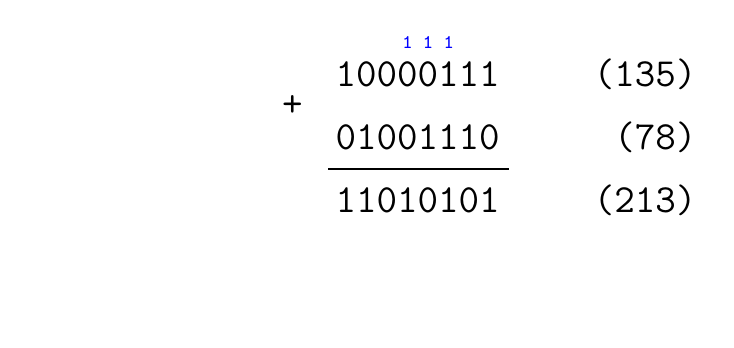
\begin{tikzpicture}
        \node[opacity=0] at (0, 0) { };

        \node[anchor=east] at (5.55, 3.4) { \scriptsize \textcolor{blue}{\texttt{1  1  1  }} };
        \node[anchor=east] at (6, 3) { \Large \texttt{10000111} };
        \node[anchor=east] at (8.5, 3) { \Large \texttt{(135)} };
        \node[anchor=east] at (6, 2.2) { \Large \texttt{01001110} };
        \node[anchor=east] at (8.5, 2.2) { \Large \texttt{(78)} };
        \node[anchor=east] at (3.5, 2.6) { \Large \texttt{+} };

        \draw[thick] (3.7, 1.8) -- (6, 1.8);

        \node[anchor=east] at (6, 1.4) { \Large \texttt{11010101} };
        \node[anchor=east] at (8.5, 1.4) { \Large \texttt{(213)} };
    \end{tikzpicture}

\end{frame}

\begin{frame}[fragile]{Overflow}

    \begin{itemize}
        \item Nas linguagems de programação, o número de \textit{bits} usados na representação
            de inteiros é limitado

        \item Por exemplo, em C/C++, variáveis do tipo \code{c}{int}  ocupam, em geral, 
            32 \textit{bits} (variáveis \code{c}{long long} ocupam 64 \textit{bits})

        \item Em geral, uma variável do tipo \code{c}{int} ocupam o mesmo espaço em memória
            que uma palavra do processador

        \item Esta limitação de espaço pode levar ao \textit{overflow}: quando o limite é 
            atingido, os \textit{bits} que excedem o tamanho máximo \lq\lq transbordam\rq\rq,
            ficando apenas aqueles dentro do limite

        \item O \textit{overflow} pode levar a resultados inesperados, e deve ser tratado com
            cuidado e atenção

    \end{itemize}

\end{frame}

\begin{frame}[fragile]{Visualização do \textit{overflow} em variáveis de 8 \textit{bits}} 

    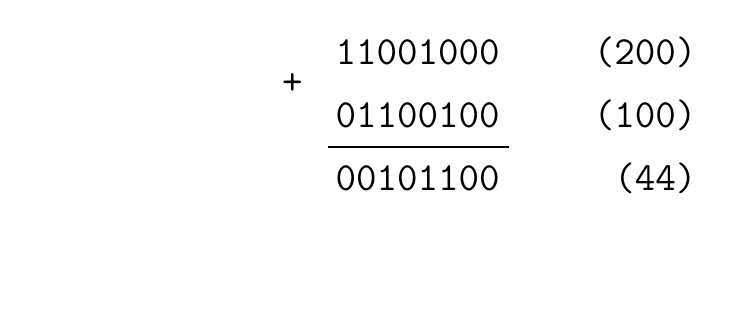
\begin{tikzpicture}
        \node[opacity=0] at (0, 0) { };

        \node[anchor=east] at (6, 3) { \Large \texttt{11001000} };
        \node[anchor=east] at (8.5, 3) { \Large \texttt{(200)} };
        \node[anchor=east] at (6, 2.2) { \Large \texttt{01100100} };
        \node[anchor=east] at (8.5, 2.2) { \Large \texttt{(100)} };
        \node[anchor=east] at (3.5, 2.6) { \Large \texttt{+} };

        \draw[thick] (3.7, 1.8) -- (6, 1.8);

        \node[anchor=east] at (6, 1.4) { \Large \texttt{00101100} };
        \node[anchor=east] at (8.5, 1.4) { \Large \texttt{(44)} };
    \end{tikzpicture}

\end{frame}

\begin{frame}[fragile]{Representação binária de números negativos}

    \begin{itemize}
        \item Para representar número negativos, utiliza-se o fato de que $n + (-n) = 0$

        \item Assim, a representação de $(-n)$ seria um número tal que, somado com $n$, daria
            resto zero

        \item Devido ao \textit{overflow}, tal número existe e é denominado complemento de 
            dois de $n$

        \item Por exemplo, em variáveis de 8 \textit{bits} de tamanho, o complemento de dois 
            de $77$ é $179$, pois $77 + 179 = 256 = 0$

        \item O complemento de dois pode ser obtido diretamente, sem necessidade de uma subtração:
            basta inverter os \textit{bits} da representação binária de $n$, e somar um ao
            resultado

        \item Desta maneira, o \textit{bit} mais significativo diferencia os números positivos
        (zero) dos negativos (um)

    \end{itemize}

\end{frame}

\begin{frame}[fragile]{Visualização do complemento de dois de $77$}

    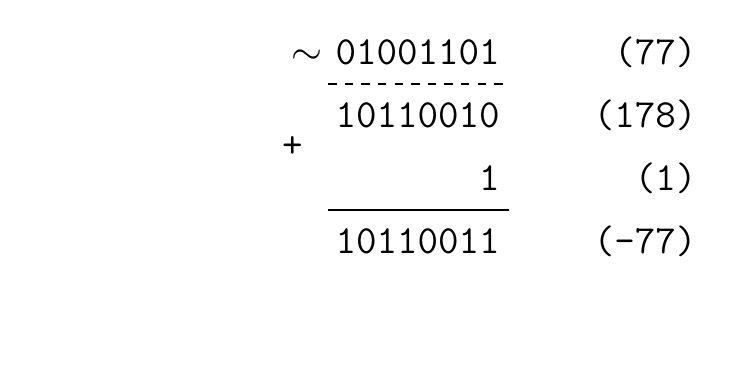
\begin{tikzpicture}
        \node[opacity=0] at (0, 0) { };

        \node[anchor=east] at (6, 3.8) { \Large $\sim$ \texttt{01001101} };
        \node[anchor=east] at (8.5, 3.8) { \Large \texttt{(77)} };
        \draw[thick,dashed] (3.7, 3.4) -- (6, 3.4);

        \node[anchor=east] at (6, 3) { \Large \texttt{10110010} };
        \node[anchor=east] at (8.5, 3) { \Large \texttt{(178)} };
        \node[anchor=east] at (6, 2.2) { \Large \texttt{1} };
        \node[anchor=east] at (8.5, 2.2) { \Large \texttt{(1)} };
        \node[anchor=east] at (3.5, 2.6) { \Large \texttt{+} };

        \draw[thick] (3.7, 1.8) -- (6, 1.8);

        \node[anchor=east] at (6, 1.4) { \Large \texttt{10110011} };
        \node[anchor=east] at (8.5, 1.4) { \Large \texttt{(-77)} };
    \end{tikzpicture}

\end{frame}


